\chapter{Data Analysis}
\section{Weighted and binary method}
\section{Pipeline}
The total number of sensors is 1056, and consequently, the same number of signals from the mattress; this leads to the necessity of an algorithm to discriminate the ones from whom it is possible to extract valuable information about the respiratory rate of the person on the mattress. A person's body can not cover the entire mattress and activate all sensors (hereafter referred to as “Channels”) simultaneously.
Many of these channels present a signal that is stationary on a value; others present just interference from the mattress. From just a few sensors, it is possible to retrieve a respiratory pattern and extract the respiratory rate per minute (rpm). Therefore becomes necessary to design a metric that underlines these channels. The meaning of this metric must be interpreted as confidence expressed as the goodness of the signal in percentual.

The designed pipeline aims to replicate a semi-realtime analysis using the data obtained during the data collection. 
For this reason, it takes in input a sliding window of 60 seconds that is moving, for each position, through the 4-minute recording.
In figure Fig. \ref{diag:pipeline} it is possible to visualize a scheme of the entire pipeline.\\



\vspace*{1.0cm}

\begin{figure}[H]
    \begin{center}
        \begin{tikzpicture}[node distance=4cm]
            %% nodi:
            \node (inizio) [box] {Awake};
            \node (stage1) [box, right of=inizio] {NREM\\Stage 1};
            \node (stage2) [box, right of=stage1] {NREM\\Stage 2};
            \node (stage3) [box, above of=stage2] {NREM\\Stage 3}; 
            \node (rem) [box, left of=stage3] {REM}; %yshift=-3cm
            %yshift=-1cm
            \draw [arrow] (inizio) -- (stage1);
            \draw [arrow] (stage1) -- (stage2);
            \draw [arrow] (stage2) -- (stage3);
            \draw [arrow] (stage3) -- (rem); % node[anchor=east] {Yes} 
            %\draw [arrow] (quest) -- ++(4,0) -- ++(0,5) -- node[] {No} (if_1);
            \draw [arrow] (rem) -- (stage1);
        \end{tikzpicture}
    \end{center}
    \caption{Pipeline}
    \label{diag:pipeline}
\end{figure}
\vspace*{1.0cm}
\subsection{Excluding criteria}
The first step of this pipeline excludes those signals for the entire window length that is stationary on value, with small amplitude, or present only interference from the mattress. So channels do not have meaningful information.
\subsubsection*{Stationary signals on a value}\label{stationary}
A stationary signal on a value is defined as a signal that remains on the same value for the entire length of the window. An example of the stationary signal on a value is shown in Fig. \ref{fig:stationaryTotal}, in this case, the channel, for this window, is excluded.
However, since it is used as a moving window it will take again into account in the next window and, if it presents a different behaviour, it maybe is considered. 
Nevertheless, If the channel presents only a part of the signal stationary on a value as in Fig. \ref{fig:spikePartial}, the channel is given as a percentage of confidence, the percentage of the non-stationary on a value signal.
\vspace*{0.5cm}
\begin{figure}[H]
    \centering
    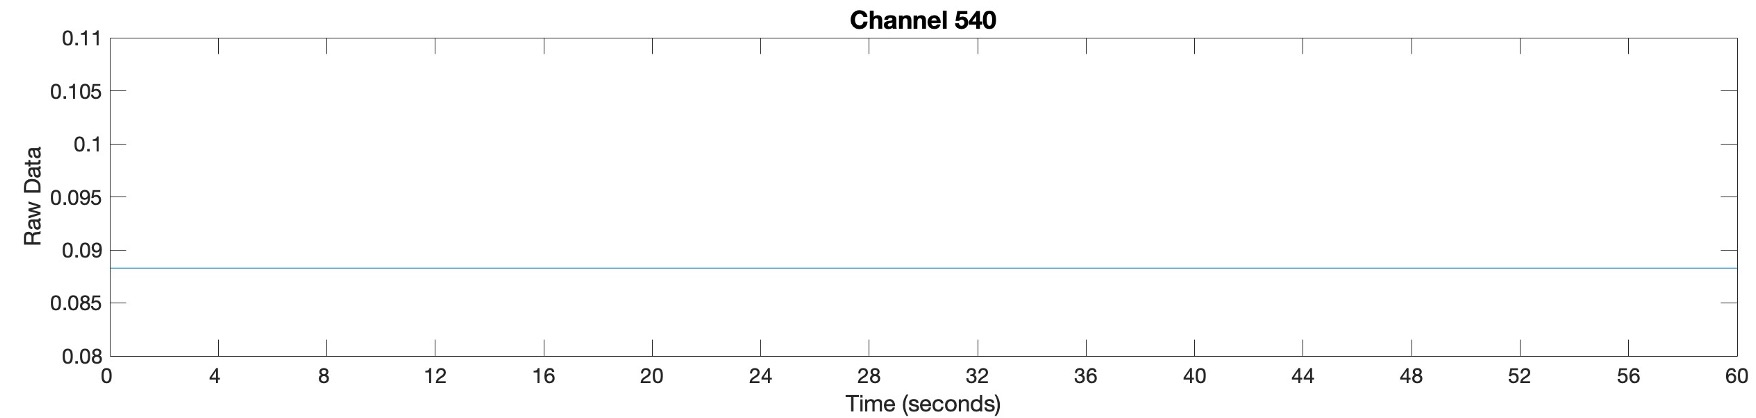
\includegraphics[width=\textwidth]{img/stationaryTotal.jpg}
    \caption{Stationary Signal}
    \label{fig:stationaryTotal}
\end{figure}
\vspace*{1.0cm}

\begin{figure}[H]
    \centering
    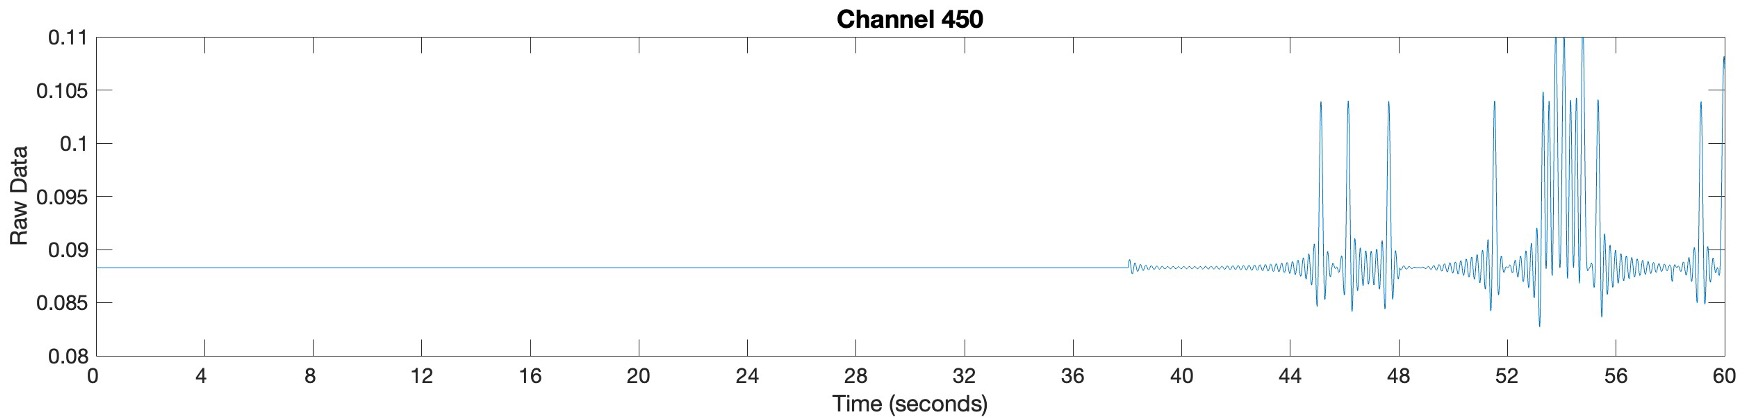
\includegraphics[width=\textwidth]{img/spakePartial.jpg}
    \caption{Spike Signal}
    \label{fig:spikePartial}
\end{figure}
\vspace*{1.0cm}

\subsubsection*{Signal with small amplitude}\label{noisy}

Several channels present a signal with a small amplitude, between [intervall], an example is visible in Fig. \ref{fig:noisy}, so after verifying if they are not stationary on a value case (Chapter \ref{stationary}), if the signal present only a noisy signal for the entire length of the window is excluded. 
Otherwise, if part of the signal is not noisy is given as a percentage of confidence, the percentage of the non-noisy signal. 
As in the previous case, due to the moving window nature of the pipeline after the shift of 10 seconds, the channel could have a different behaviour and be further analysed.\\


%\vspace*{1.0cm}
\begin{figure}[H]
    \centering
    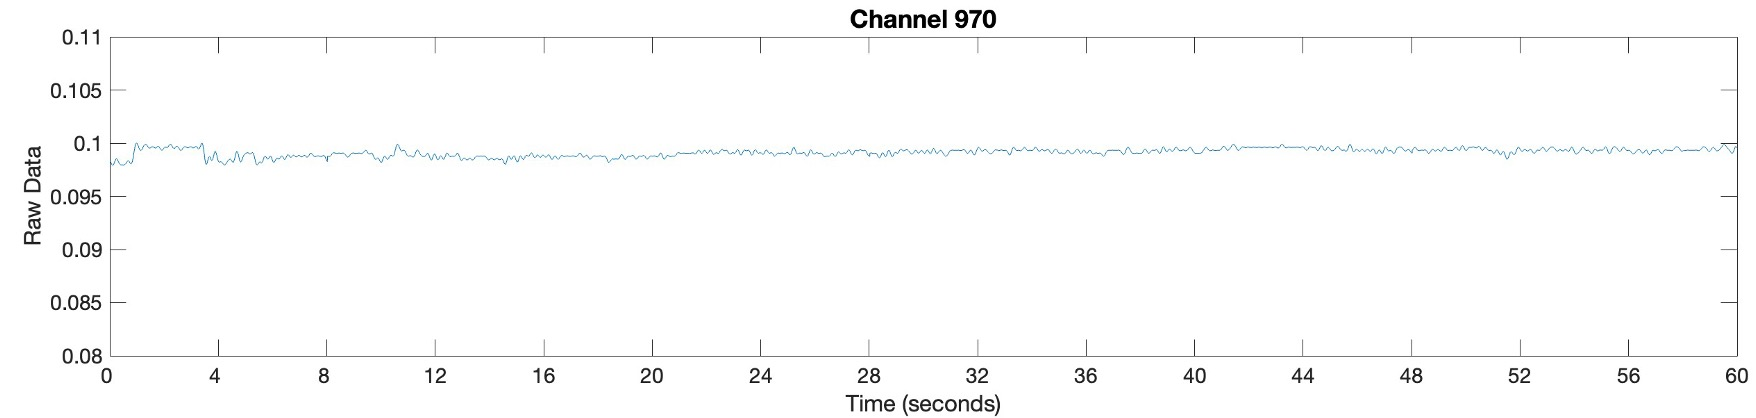
\includegraphics[width=\textwidth]{img/noisy.jpg}
    \caption{Noisy Signal}
    \label{fig:noisy}
\end{figure}


\subsubsection{Spikes Signals} \label{spikes}
The mattress can produce artefacts, that are visible in the channels as spikes as in Fig.\ref{fig:spikeTotal}. Since these artefacts are visible also in channels that present a good respiratory pattern (Fig.\ref{fig:goodSignal}), after evaluating different thresholds it has been decided to accept the channel that has a percentage of spikes under 30\%.\\


\begin{figure}[H]
    \centering
    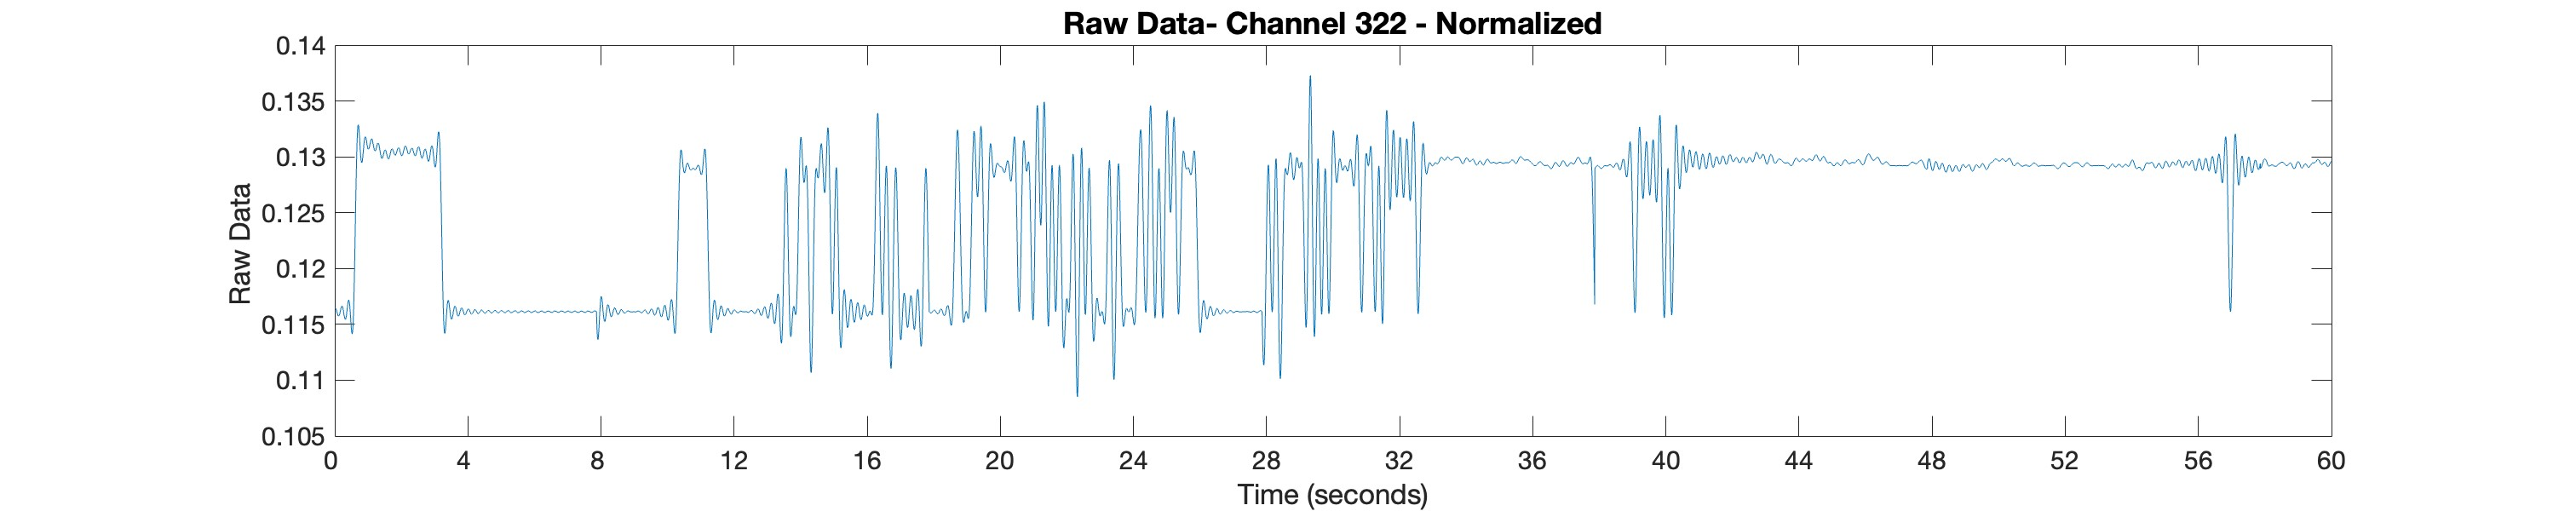
\includegraphics[width=\textwidth]{img/spike_total.jpg}
    \caption{Stationary Signal}
    \label{fig:spikeTotal}
\end{figure}

\begin{figure}[H]
    \centering
    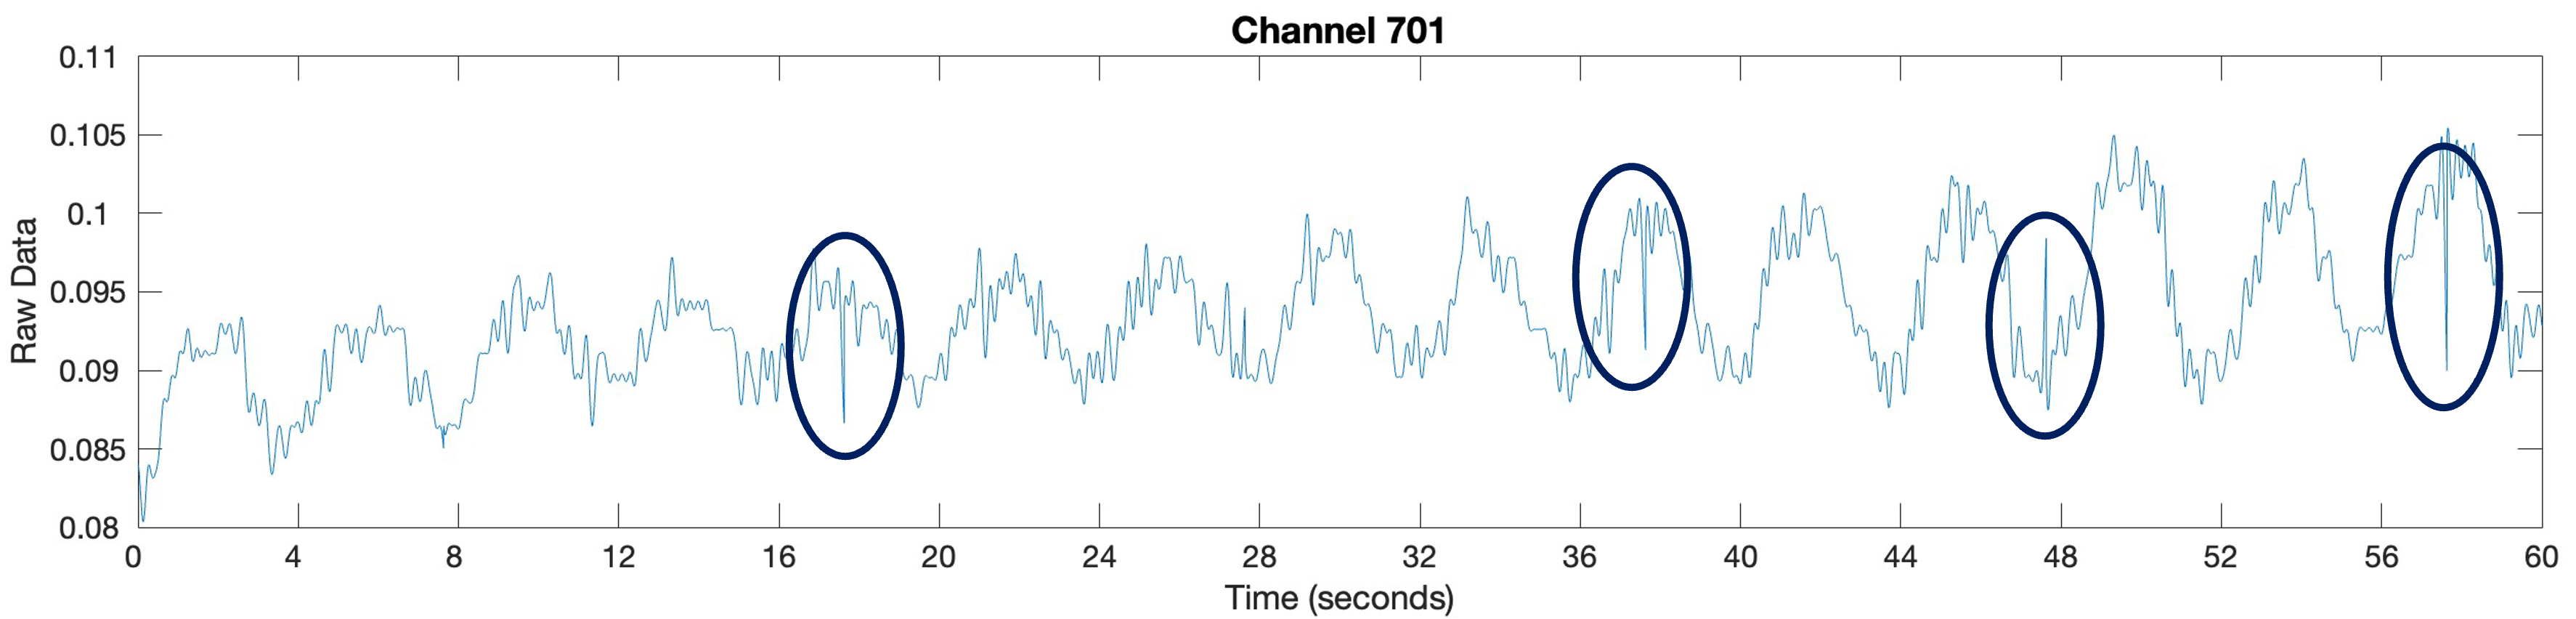
\includegraphics[width=\textwidth]{img/goodSpikes.png}
    \caption{Good signal}
    \label{fig:goodSignal}
\end{figure}

\subsection{Denoised Signals}
After these preliminary analyses, the number of signals decreases drastically; as a result, has been obtained signals that could contain valuable information and the relative percentage of confidence.
To be able to estimate the number of breaths it has been assumed to count as one breath the moment between inhale and exhale, which can also be considered a peak in the signal.
At this point, most of the signals are still noisy. To be better analysed has been decided to denoise it using two different kinds of approaches: Multiresolution analysis of the maximal overlap discrete wavelet transform (Chapter \ref{Wavelet}), and Savitz-Golay filter (Chapter \ref{sg}).

\subsection{Wavelet} \label{Wavelet}

The Multiresolution Overlap Discrete Wavelet Transform (hereafter also referred to as "MODWTMRA") is based on wavelet analysis (MOWDT) that transforms the original signal into a time-frequency domain to be analysed and processed, the multiresolution analysis (MRA), which cuts the signal into components, can produce the original signal exactly when added back together.

The input data of MOWDT are samples of a function $f(x)$ evaluated at $N$ time points, this function can be expressed as the linear combination of the scaling function $\phi(x)$ and wavelet $\psi(x)$ at varying scales and translations:

$$f(x)=\sum_{k=0}^{N-1} c_k 2^{-J_0/2} \phi(2^{-J0}x-k) + \sum_{j=1}^{J_0}f_j(x)$$
where $$f_j(x)=\sum_{k=0}^{N-1} d_{j,k}2^{-J/2} \phi(2^{-J}x-k)$$
and $J_0$ is the number of levels of wavelet decomposition calculated as $floor(log_2(N))$.

The first sum represents the first approximation of the signal and then the successive scales.
MODWT returns the $N$ coefficients $\{c_k\}$ and the $(J_0 $ X $ N)$ detail coefficients $\{d_{j,k}\}$ of the expansion. 

Since it has been used the MODWTMRA, instead of just MODWT, the returns is the projections of the function $f(x)$ onto the various wavelet subspaces and final scaling space. That is, MODWTMRA returns 
$$\sum_{k=0}^{N-1} c_k 2^{-J_0/2} \phi(2^{-J0}x-k)$$\newline
and the $J_0$-many $\{f_j(x)\}$ evalutaed at $N$ time points.
It is then obtained a projection of $f(x)$ onto a different subspace, the original signal can be recovered by adding all the projections. 

For our approach, we choose the Daubechies wavelet with two vanishing moments (Fig.\ref{fig:Daubechies}) that better represent the breath signal present in our data.

\begin{figure}[h]
    \centering
    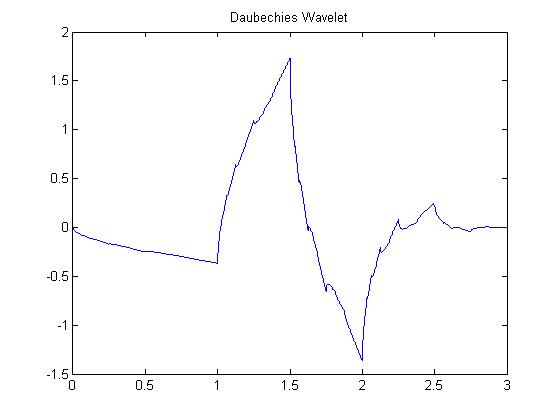
\includegraphics[width=0.6\textwidth]{img/gooddb.jpeg}
    \caption{Daubechies wavelet with two vanishing moments}
    \label{fig:Daubechies}
\end{figure}

In figure Fig. \ref{fig:level1} is possible to visualize the decomposition of a channel

To obtain our denoised signal, it has been decided to sum only a subset of this scale, which allowed us to reconstruct a clear signal where the peaks could be underlined and counted. 

In figure Fig. \ref{fig:level1} is possible to visualize the decomposition of a channel, the raw data of which is being viewed in the first plot of that image, it has been decomposed in 13 levels. \\



\begin{figure}[p]
    \centering
    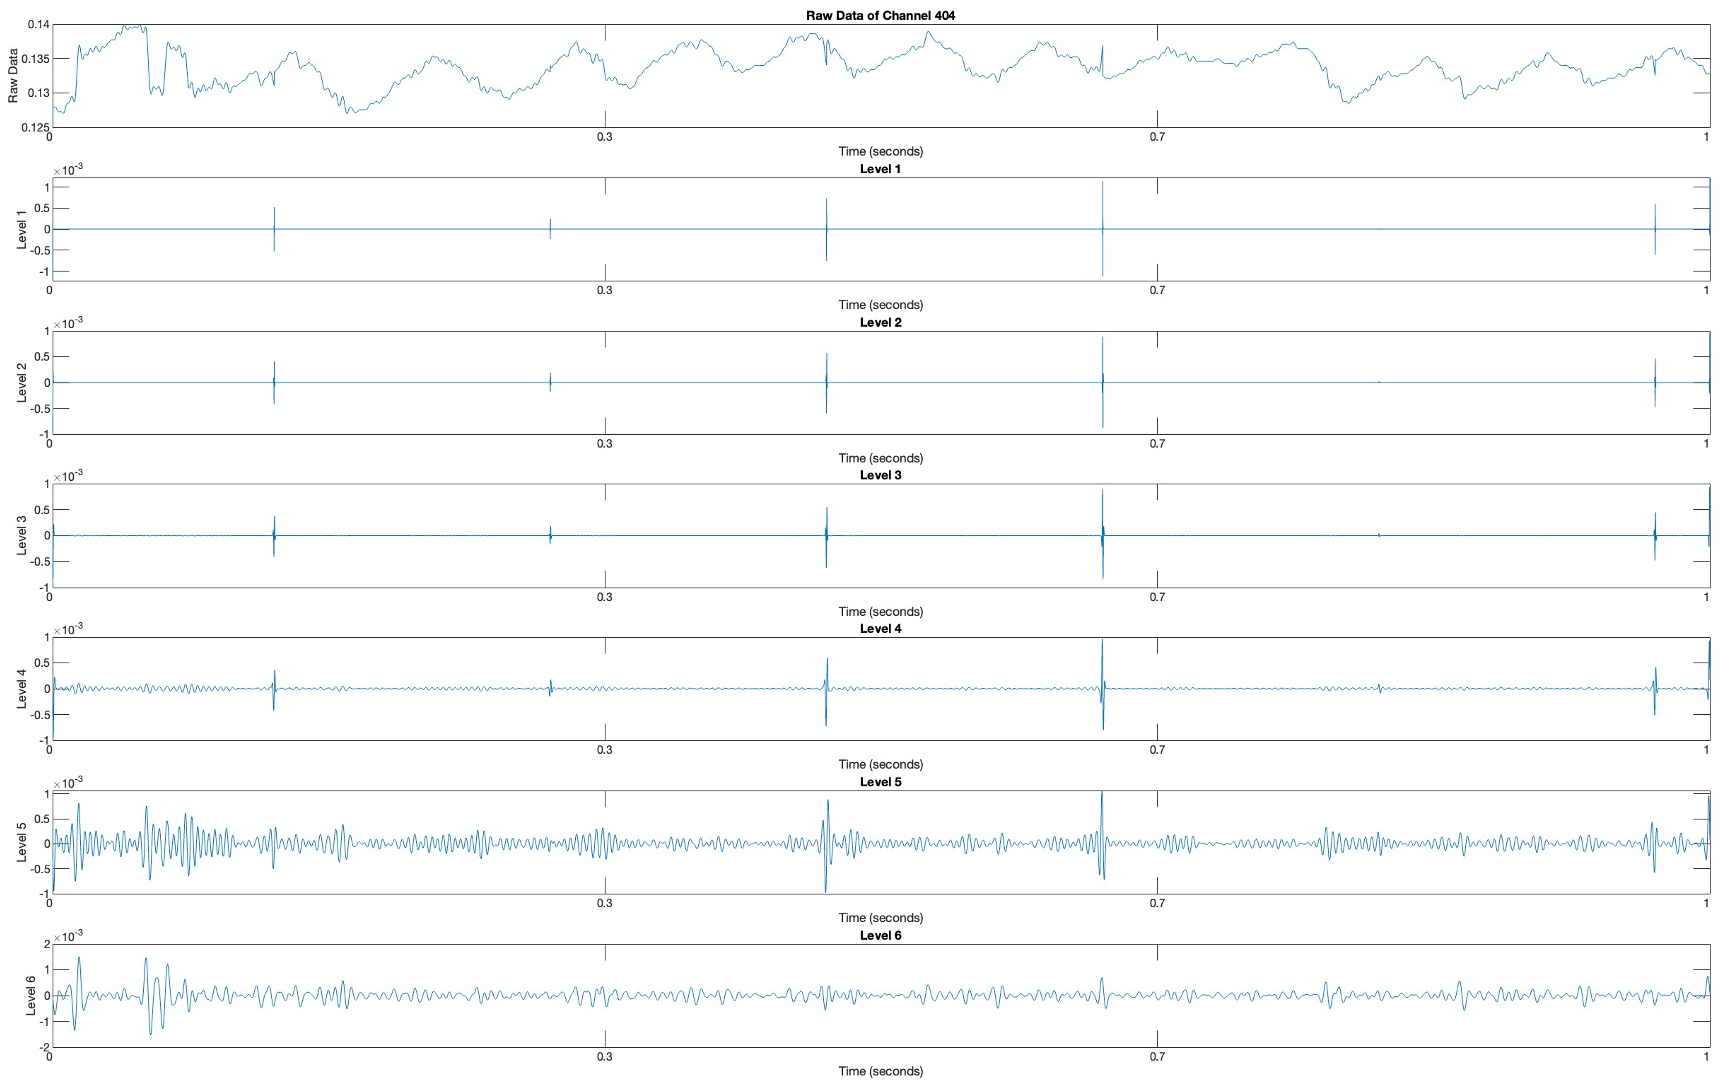
\includegraphics[width=\textwidth]{img/lev1.png}
    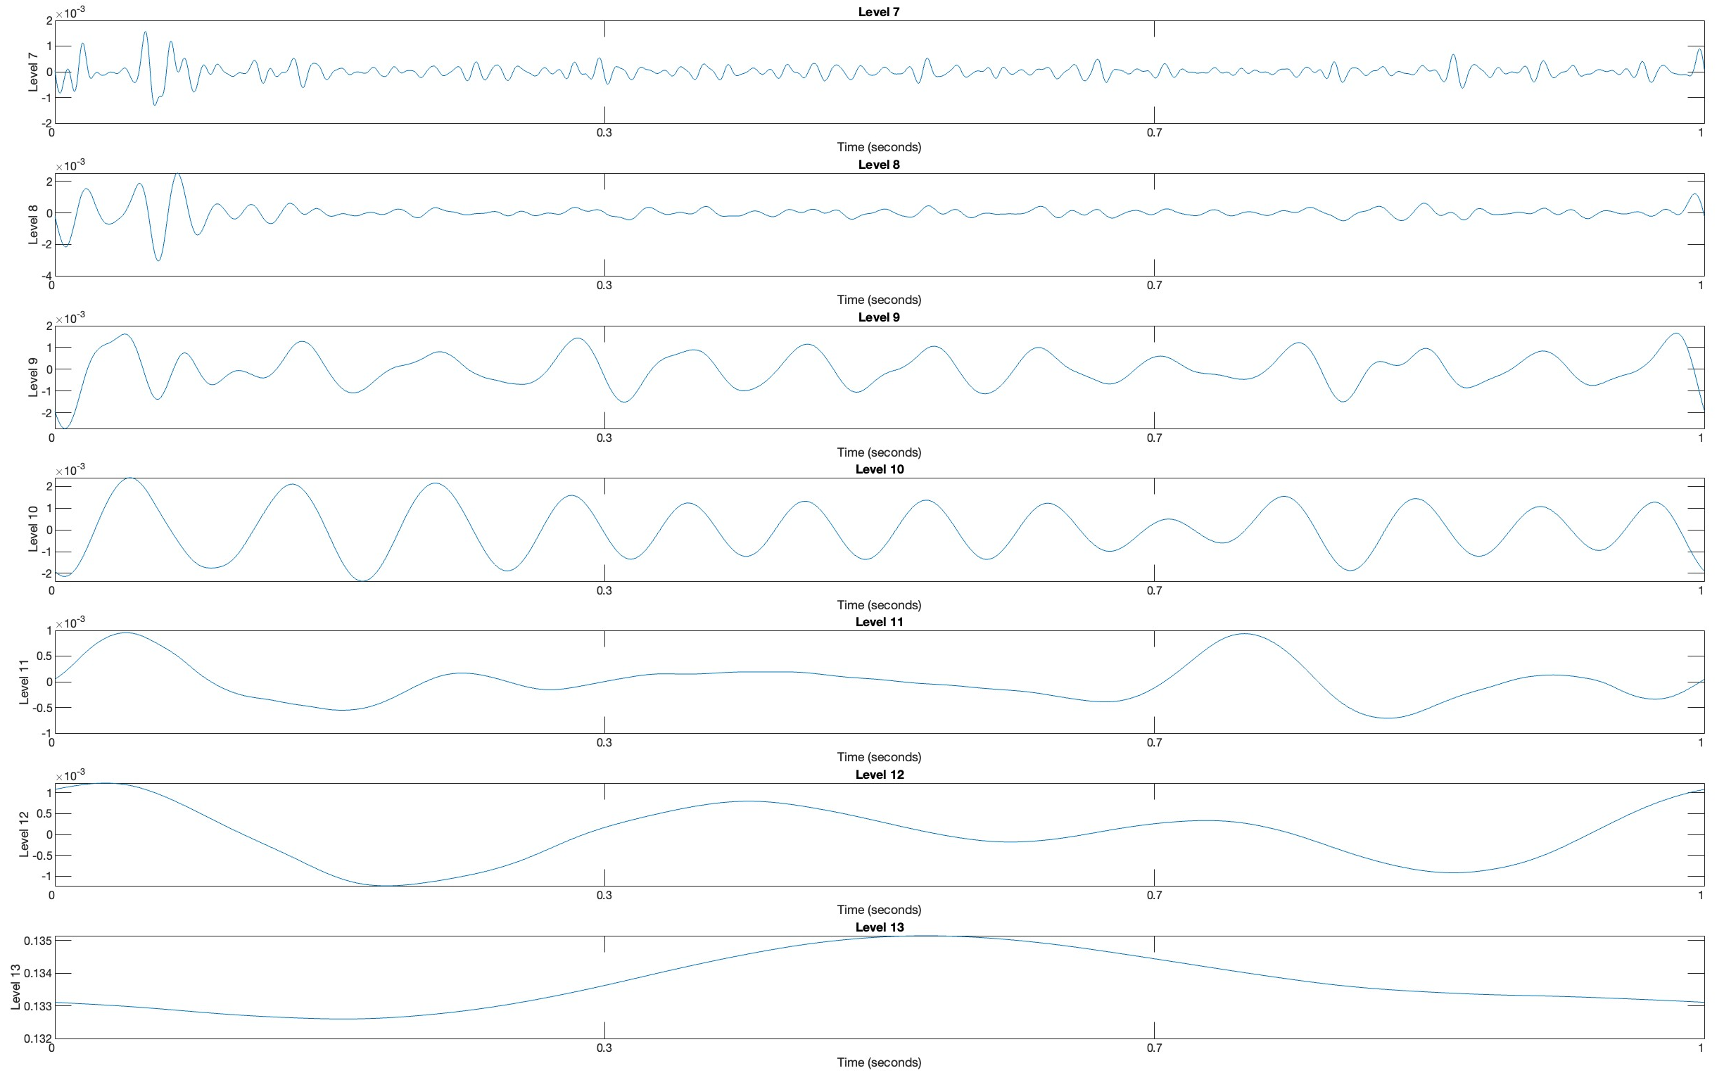
\includegraphics[width=\textwidth]{img/lev2.png}
    \caption{Stationary Signal}
    \label{fig:level1}
\end{figure}


\begin{comment}



Wavelet analysis is based on the decomposition of a signal into ``scales'' using a wavelet, for our approach, it has been choosing the Daubechies wavelet with two vanishing moments better represent the breath signal present in our data. The temporal analysis is performed with a contracted, high-frequency version of the wavelet, while the frequency analysis is performed with dilated ones.

 Wavelets are functions that satisfy the requirements of both time and frequency localization and are also orthogonal to each other.
\end{comment}







\begin{comment}
    The generated waveforms are analyzed with Wavelet multiresolution analysis (MRA) to extract subband information from the simulated transients. Daubechies Eight (D-8) wavelet is used in this work for the analysis as it closely matches the signal to be processed which is of utmost importance in wavelet applications. Also, the \cite{1273161}
\end{comment}
\subsubsection{using in the thesis}
\subsection{Savitz-Golay filter} \label{sg}


The Savitz-Golay filter is a filter used to "smooth out" a noisy signal whose frequency span (without noise) is significant. 
They are also called digital smoothing polynomial filters or least-squares smoothing filters. 
In general, filtering consists of replacing each point of a signal by some combination of the signal values contained in a moving window centered at the point, on the assumption that nearby points measure nearly the same underlying value. 
Savitzky-Golay filters generalize this idea by least-squares fitting an nth-order polynomial through the signal values in the window and taking the calculated central point of the fitted polynomial curve as the new smoothed data point.
\begin{comment}
The idea of Savitzky-Golay filters is that each sample in the filtered sequence takes its direct neighbourhood of N neighbours and fits a polynomial to it.
\end{comment}

So, in the end, is possible to obtain a wave similar to the one in MODWTMRA form, which is likely to count the peaks, interpreted as the rpm.\\
\subsubsection{theory}
\subsubsection{using in the thesis}

 


\subsection{SNR ratio}

\subsection{Subsequent analyses of the filtered signal}


The so reconstructed signals were given as input to a pick finder to select both peaks and valleys of the signal. 
We then exclude the channels with a signal with more than 30 rpm because the normal rpm during sleep is between 8-25 rpm, but since over 20 is predictive of cardiopulmonary arrest, we decide to keep only signals under 30 rpm.

The remaining signals are further analyzed in their structure: via Euclidean distance between the signal's valley and peaks should differ by up to ±20$\%$ from the preceding breath, and also via the distance between peaks and valleys on the time axis that should vary between ±20 \% from the previous breath.
These two last analysis also gives a percentage of confidence that the signal recreates a breath pattern.

In the end, to calculate the rpm, the channels with the highest accuracy are taken into account, and the rpm is computed as the average of the number of peaks of the signals.
It is also possible to visualize a heatmap to understand where the best channel is in respect of the body. 

\subsection{Result of the Pipeline (visual)}